\newif\ifshowsolutions
% \showsolutionstrue
\documentclass{article}
\usepackage{listings}
\usepackage{amsmath}
\usepackage{subfig}
\usepackage{amsthm}
\usepackage{amsmath}
\usepackage{amssymb}
\usepackage{graphicx}
\usepackage{mdwlist}
\usepackage{geometry}
\usepackage{titlesec}
\usepackage{palatino}
\usepackage{mathrsfs}
\usepackage{fancyhdr}
\usepackage{paralist}
\usepackage{todonotes}
\usepackage{tikz}
\usepackage{float} % Place figures where you ACTUALLY want it
\usepackage{comment} % A hack to toggle sections
\usepackage{ifthen}
\usepackage{mdframed}
\usepackage{verbatim}
\usepackage{listings}
\usepackage{bbm}
\usepackage{upquote} % Prevents backticks replacing single-quotes in verbatim
\usepackage[strings]{underscore}
\usepackage[colorlinks=true]{hyperref}
\usetikzlibrary{positioning,shapes,backgrounds}

\geometry{margin=1in}
\geometry{headheight=2in}
\geometry{top=2in}

\setlength{\marginparwidth}{2.15cm}
\setlength{\parindent}{0em}
\setlength{\parskip}{0.6\baselineskip}

\rhead{}
\lhead{}

% Spacing settings.
\titlespacing\section{0pt}{12pt plus 2pt minus 2pt}{0pt plus 2pt minus 2pt}
\titlespacing\subsection{0pt}{12pt plus 4pt minus 2pt}{0pt plus 2pt minus 2pt}
\titlespacing\subsubsection{0pt}{12pt plus 4pt minus 2pt}{0pt plus 2pt minus 2pt}
\renewcommand{\baselinestretch}{1.15}

% Shortcuts for commonly used operators.
\newcommand{\E}{\mathbb{E}}
\newcommand{\Var}{\operatorname{Var}}
\newcommand{\Cov}{\operatorname{Cov}}
\newcommand{\Bias}{\operatorname{Bias}}
\DeclareMathOperator{\argmin}{arg\,min}
\DeclareMathOperator{\argmax}{arg\,max}

% Do not number subsections and below.
\setcounter{secnumdepth}{1}

% Custom format subsection.
\titleformat*{\subsection}{\large\bfseries}

% Set up the problem environment.
\newcounter{problem}[section]
\newenvironment{problem}[1][]
  {\begingroup
    \setlength{\parskip}{0em}
    \refstepcounter{problem}\par\addvspace{1em}\textbf{Problem~\Alph{problem}\!
    \ifthenelse{\equal{#1}{}}{}{ [#1 points]}:}
  \endgroup}

% Set up the subproblem environment.
\newcounter{subproblem}[problem]
\newenvironment{subproblem}[1][]
  {\begingroup
    \setlength{\parskip}{0em}
    \refstepcounter{subproblem}\par\medskip\textbf{\roman{subproblem}.\!
    \ifthenelse{\equal{#1}{}}{}{ [#1 points]:}}
  \endgroup}

% Set up the teachers and materials commands.
\newcommand\teachers[1]
  {\begingroup
    \setlength{\parskip}{0em}
    \vspace{0.3em} \textit{\hspace*{2em} TAs responsible: #1} \par
  \endgroup}
\newcommand\materials[1]
  {\begingroup
    \setlength{\parskip}{0em}
    \textit{\hspace*{2em} Relevant materials: #1} \par \vspace{1em}
  \endgroup}

% Set up the hint environment.
\newenvironment{hint}[1][]
  {\begin{em}\textbf{Hint: }}
  {\end{em}}


% Set up the solution environment.
\ifshowsolutions
  \newenvironment{solution}[1][]
    {\par\medskip \begin{mdframed}\textbf{Solution~\Alph{problem}#1:} \begin{em}}
    {\end{em}\medskip\end{mdframed}\medskip}
  \newenvironment{subsolution}[1][]
    {\par\medskip \begin{mdframed}\textbf{Solution~\Alph{problem}#1.\roman{subproblem}:} \begin{em}}
    {\end{em}\medskip\end{mdframed}\medskip}
\else
  \excludecomment{solution}
  \excludecomment{subsolution}
\fi


\usepackage{url}


\chead{%
  {\vbox{%
      \vspace{2mm}
      \large
      Machine Learning \& Data Mining \hfill
      Caltech CS/CNS/EE 155 \hfill \\[1pt]
      Final Exam \hfill
      March 15th, 2020 \\
    }
  }
}
\newcommand{\fh}{\hat{f}}
\newcommand{\St}{\tilde{\Sigma}}
\newcommand{\Zt}{\tilde{Z}}
\newcommand{\Xt}{\tilde{X}}
\newcommand{\tr}{\texttt{trace}}
\newcommand{\yh}{\hat{y}}
\newcommand{\fb}{\bar{f}}


\begin{document}
\pagestyle{fancy}

\begin{itemize}
\item Due noon, March 24th, via Gradescope.
\item No extensions, and you cannot use late hours.
\item No collaboration, you must answer these questions all on your own.
\item You are free to ask clarification questions on Piazza.
\item This exam is designed to take 3-5 hours to do.
\item Suggestion: Write the solutions by hand (no LaTeX) and submit a scanned copy.  It will save you time.
\item All questions have short answers.  If your answer is very long, you're probably over-thinking it.
\end{itemize}
\medskip


\newpage

\section{Multiple Choice Questions (35 points) }

Just specify the correct answer.  No need to justify.

\subsection{Lasso (2 points)}

\question (True or False) Every L1-constrained regression problem is equivalent to some L1-regularized regression problem.

Recall that an L1-constrained regression problem is:
$$\argmin_{w,b} \sum_{(x,y)\in S} \left(y - (w^Tx + b)\right)^2,\ \ \ \      \mbox{s.t.}\ \ \ \ \ \|w\|_1 \leq C,
$$
and that an L1-regularized regression problem is:
$$\argmin_{w,b} \lambda\|w\|_1 + \sum_{(x,y)\in S} \left(y - (w^Tx + b)\right)^2.$$

\vspace{-0.2in}
\begin{solution}
True
\end{solution}

%\smallskip

\subsection{Bagging \& Bootstrap Sampling (3 points)}

\question
(Multiple Choice) Suppose we generate $M$ bootstraps $S'_1,\ldots,S'_M$ of a training set $S=\{(x_i,y_i)\}_{i=1}^N$.  For any specific $(x,y) \in S$, what is the probability that $(x,y)$ does not appear in ANY of $S'_1,\ldots,S'_M$?

(Recall that a bootstrap is a dataset with the same size as $S$ generated by sampling uniformly with replacement from $S$.)
%\smallskip

\textbf{Option A:}
$$
\left(1-\frac{1}{N}\right)^NM
$$
%\smallskip

\textbf{Option B:}
$$
\left(1-\frac{1}{N}\right)^{NM}
$$
%\smallskip

\textbf{Option C:}
$$
\left(1-\frac{1}{NM}\right)^{NM}
$$
%\smallskip

\textbf{Option D:}
$$
\left(1-\left(1-\frac{1}{NM}\right)^N\right)^M
$$
%\smallskip

\vspace{-0.2in}
\begin{solution}
B
\end{solution}

%\smallskip


\newpage

\subsection{Convolutional Filters (4 points)}


Consider the three convolutional filters below:

\begin{small}
\[K_{1} = \begin{bmatrix}
0.0043 & 0.0144 & 0.0214 & 0.0144 & 0.0043 \\
0.0144 & 0.0478 & 0.0712 & 0.0478 & 0.0144 \\
0.0214 & 0.0712 & 0.1062 & 0.0712 & 0.0214 \\
0.0144 & 0.0478 & 0.0712 & 0.0478 & 0.0144 \\
0.0043 & 0.0144 & 0.0214 & 0.0144 & 0.0043 
\end{bmatrix}\]

\[K_{2} = \begin{bmatrix}
0.0068 & 0.0225 & 0.0335 & 0.0225 & 0.0068 \\
0.0225 & 0.0746 & 0.1112 & 0.0746 & 0.0225 \\
0.0335 & 0.1112 & 0.1660 & 0.1112 & 0.0335 \\
0.0225 & 0.0746 & 0.1112 & 0.0746 & 0.0225 \\
0.0068 & 0.0225 & 0.0335 & 0.0225 & 0.0068 
\end{bmatrix}\]

\[K_{3} = \begin{bmatrix}
0 & 0 & 0 & 0 & 0\\
0 & 0 & 0 & 0 & 0\\
0 & 0 & 0.8 & 0 & 0\\
0 & 0 & 0 & 0 & 0\\
0 & 0 & 0 & 0 & 0
\end{bmatrix}\]
\end{small}

\question (Multiple Choice) If we apply $K_1$, $K_2$, and $K_3$ to Figure \ref{fig:convolve0}, which filter corresponds to which  image in Figure \ref{fig:convolve}?

\smallskip


\begin{figure}[h]
\vspace{-0.2in}
        \centering
	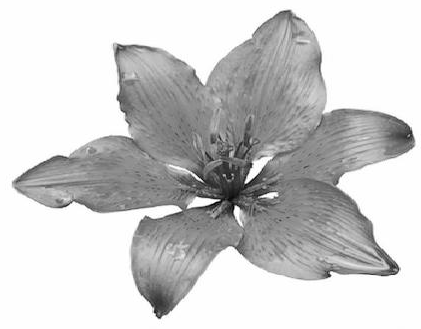
\includegraphics[scale=0.3]{image/white_black.png}
   \vspace{-0.1in}
   \caption{Original Image.  All pixel intensities are clipped between 0 and 1 (black=0 and white=1).}
\label{fig:convolve0}
   \end{figure}
   \begin{figure}[h]
\vspace{-0.2in}
   \centering
			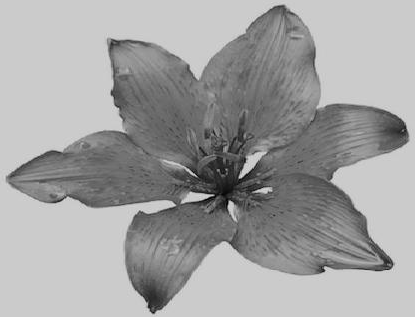
\includegraphics[scale=0.304]{image/darken.png}~~
			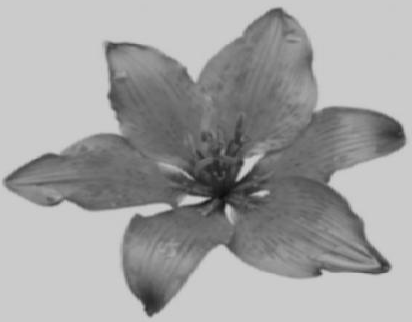
\includegraphics[scale=0.3]{image/dark_blur.png}~~
			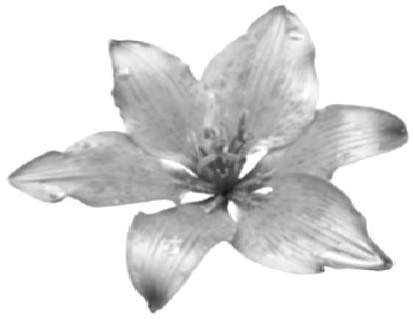
\includegraphics[scale=0.3]{image/brighten_blur.png}
   \vspace{-0.1in}
         \caption{Convolved Images (hint: the grey background is intentional)}
\label{fig:convolve}
\end{figure}

\vspace{-0.2in}
\begin{solution}
$K_1$ = Middle, $K_2$ = Right, $K_3$ = Left
\end{solution}


\smallskip





\subsection{Multiclass SVMs (3 points)}
\label{sec:multiclass_svm}


Consider the following 4-class multiclass SVM objective:
\begin{align*}
&\argmin_{w,\xi} \frac{1}{2}\|w\|^2 + \frac{C}{N}\sum_{i=1}^N \xi_i\\
\mbox{s.t.}\\
   & \forall i, \forall y' \in \{1,2,3,4\}:\ w_{y_i}^T x_i - w_{y'}^Tx_i \geq \textbf{1}_{[y_i\neq y']} - \xi_i
\end{align*}
where:
$$ w = \left[\begin{array}{c}
w_1\\
w_2\\
w_3\\
w_4
\end{array}\right],$$
and predictions are made via $\argmax_{y} w_y^Tx$.  In other words, each $\xi_i$ can be defined as:
\begin{eqnarray}
\xi_i = \max_{y' \in \{1,2,3,4\}} \left\{\textbf{1}_{[y_i\neq y']} - \left(w_{y_i}^T x_i - w_{y'}^Tx_i\right)\right\}\label{eqn:xi}.
\end{eqnarray}

Suppose for training data $(x_i,y_i)$ we have $y_i = 1$ and:
$$w_1^Tx_i  = 1.0,$$
$$w_2^Tx_i  = 1.5,$$
$$w_3^Tx_i  = 0.1,$$
$$w_4^Tx_i  = -0.8.$$

\smallskip

\question (Multiple Choice) Which $\yh\in\{1,2,3,4\}$  is the maximizer of \eqref{eqn:xi}?


\begin{solution}
$\yh = 2$
\end{solution}

\smallskip

\subsection{Feature Maps (3 points)}

Consider the following 3-class multiclass feature map:
\begin{eqnarray}
\phi(x,y) = \left[\begin{array}{c}
\textbf{1}_{[y=1]} x\\
\textbf{1}_{[y=2]} x\\
\textbf{1}_{[y=3]} x\\
-\textbf{1}_{[y\in\{1,2\}]} x
\end{array}\right],
   \label{eqn:feature}
   \end{eqnarray}
where predictions are made via $\argmax_{y\in\{1,2,3\}} w^T\phi(x,y)$.

\question (Multiple Choice) What is the effect of using \eqref{eqn:feature} versus a ``conventional'' multiclass feature map of:
\begin{eqnarray}
\phi(x,y) = \left[\begin{array}{c}
\textbf{1}_{[y=1]} x\\
\textbf{1}_{[y=2]} x\\
\textbf{1}_{[y=3]} x\\
\end{array}\right].
   \label{eqn:feature2}
   \end{eqnarray}

\textbf{Option A:} Compared to \eqref{eqn:feature2}, in \eqref{eqn:feature} the model scores for Class 1 \& 2 are encouraged to be correlated.
\smallskip

\textbf{Option B:} Compared to \eqref{eqn:feature2}, in \eqref{eqn:feature} the model scores for Class 1 \& 2 are encouraged to be anti-correlated.
\smallskip

\textbf{Option C:} Either A or B are possible depending on the specific training data.
\smallskip

(Recall that the model score for a class $y'$ is just $w^T\phi(x,y')$.)

\begin{solution}
A
\end{solution}

\smallskip

\subsection{Hard-Margin SVMs (5 points)}

A hard margin SVM can be written as:
%\begin{align*}
%& \argmin_{w,b} \frac{1}{2}\|w\|^2\\
%\mbox{s.t.}\\
%& \forall (x,y)\in S: y(w^T x -b) \geq 1
%\end{align*}
\begin{figure}[h]
\vspace{-0.12in}
\centering
%\includegraphics[scale=0.3]{image/svm.pdf}
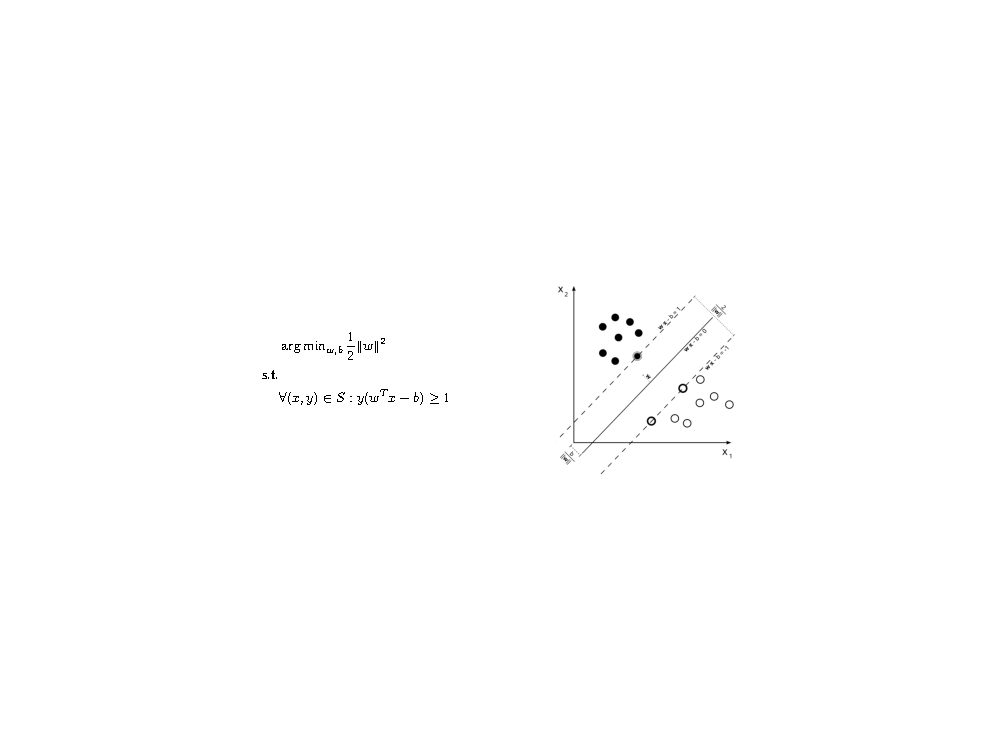
\includegraphics[scale=1.65]{image/svm2.pdf}
\vspace{-0.1in}
\end{figure}

The figure to the right depicts a visualization of the hard-margin SVM for a 2-dimensional example (image source Wikipedia).  The data points that are on the margin (for which the inequality constraint in the training optimization problem is a tight equality) are known as ``support vectors''.


\question (True or False) If the data is not linearly separable, then a hard-margin SVM returns $w=0$.  

\begin{solution}
False
\end{solution}


\smallskip 



\question (Multiple Choice) Assume the data is linearly separable. What happens when we remove a data point that is NOT a support vector from the training set, and then retrain the model?

\smallskip

\textbf{Option A:} The solution $w$ and $b$ do not change from before.
\smallskip

\textbf{Option B:} The solution changes, and the training error is reduced.
\smallskip

\textbf{Option C:} The solution changes, and the training error is increased.
\smallskip

\vspace{-0.1in}
\begin{solution}
A
\end{solution}

\subsection{AdaBoost (2 points)}
\question (True or False)  Each iteration of AdaBoost is guaranteed to reduce the training 0/1 Loss of the aggregate model. 

Recall that the aggregate model of AdaBoost at iteration $T$ is:
$$f_T(x) = \sum_{t=1}^T \alpha_t h_t(x)\in\Re,$$
and predictions are made via the sign of $f_T(x)$: $h_T(x) = \texttt{sign}(f_T(x))$.  %Also recall that the Exponential Loss of a data point $(x,y)$ with $y \in \{-1,+1\}$ is
%$$L(y,f_T(x)) = \exp\left\{-yf_T(x)\right\}.$$


\vspace{-0.1in}
\begin{solution}
False
\end{solution}

\smallskip

\subsection{Tensor Model Training (2 points)}

\question (True or False) Every L2-regularized tensor latent-factor regression problem can be optimized via alternating closed-form optimization (i.e., converges to a local optimum).

Recall that a L2-regularized tensor regression problem can be written as:
$$\argmin_{U,V,W} \frac{1}{2}\left(\|U\|_F^2 + \|V\|_F^2 + \|W\|_F^2\right) + \frac{1}{2}\sum_{(a,b,c)\in S}\left(Y_{a,b,c} - \langle u_a,v_b,w_c\rangle\right)^2,$$
where  $u_a$, $v_b$, and $w_c$ correspond to the $a$-th column of $U$, the $b$-th column of $V$, and the $c$-th column of $W$, respectively.  The three-way dot product is defined as:
$$\langle u_a,v_b,w_c\rangle = \sum_{k=1}^K u_{a,k}v_{b,k}, w_{c,k}.$$
Alternating closed-form optimization implies that $U$ (likewise $V$ or $W$) can be solved optimally in closed-form if one holds the other two matrices $V$ and $W$ fixed.


\vspace{-0.1in}
\begin{solution}
True
\end{solution}

\smallskip

\subsection{Bias-Variance Decomposition (2 points)}

Let $f_S \in F_S$ denote a set of linear regression models  trained on training set $S$ using different learning algorithms (e.g., each $f_S$ is  trained using a different regularization strength).
Let $\fh_S$ denote the $f_S \in F_S$ that has the lowest bias  in the bias-variance decomposition.

\question (True or False)  The minimum bias learning algorithm is guaranteed to have the smallest test squared loss.  In other words, the test error of $\fh_S$ is guaranteed to be lower than the test error of any other $f_S$:
$$\forall f_S \in F_S:\ E_{(x,y)\sim P(x,y)} E_{S}\left[\left(y-\fh_S(x)\right)^2\right] \leq E_{(x,y)\sim P(x,y)} E_{S}\left[(y-f_S(x))^2\right],$$
where $P(x,y)$ denotes the test distribution.

\begin{solution}
False
\end{solution}

\smallskip

\subsection{HMM EM Learning (3 points)}

\question
(Multiple Choice)
During EM training in the unsupservised setting, what best describes what happens when you initialize $P(y^j|y^{j-1})$ and $P(x^j|y^j)$ to both be the uniform distribution?

\smallskip

\textbf{Option A:}  Nothing special, you just converge to some local optimum.
\smallskip

\textbf{Option B:}  You converge to a degenerate local optimum where all the hidden states learn the same thing.
\smallskip

\textbf{Option C:}  You get a divide-by-0 error and training crashes.
\smallskip

Recall that an HMM model is specified by:
$$P(x,y) = P(End|y^M)\prod_{j=1}^M P(x^j|y^j)P(y^j|y^{j-1}),$$
the unsupervised learning problem is specified by
$$\argmax_{\Theta} \prod_{x\in S} P(x) = \argmax_{\Theta} \prod_{x\in S} \sum_{y'} P(x,y'),$$
where $S$ denotes the training set and $\Theta$ denotes all the HMM model parameters. 
The EM algorithm alternates between inferring the distribution of sequences $y'$ for each training example $x$ and using that inferred distribution to estimate better model parameters $\Theta$.  


\begin{solution}
B
\end{solution}



\subsection{Non-Negative Matrix Factorization (2 points)}

Consider the matrix factorization problem of minimizing squared reconstruction error:
$$\argmin_{U\in \Re^{N\times K}, V\in \Re^{M\times K}} \|Y - UV^T\|_{Fro}^2,$$
where $Y \in \Re^{N \times M}$ is the matrix we wish to encode in a low-rank model, and $U$ and $V$ are our model components.

\question (True or False) Suppose $Y$ is non-negative.  If we enforce $U$ and $V$ to also be non-negative, then we typically need a larger latent dimension $K$ to achieve the same squared reconstruction error compared to allowing $U$ and $V$ to take negative values.

\begin{solution}
True
\end{solution}

\subsection{Decision Trees (2 points)}

\question (True or False) Given infinite training data (sampled i.i.d. from the test distribution), decision trees can essentially learn arbitrary classifier functions. (Ignore the distinction between countably vs uncountably infinite, this is a high-level conceptual question.)

\begin{solution}
True
\end{solution}

\subsection{Overfitting (2 points)}
\question (True or False) Given infinite training data (sampled i.i.d. from the test distribution), it is essentially impossible to overfit. (Ignore the distinction between countably vs uncountably infinite, this is a high-level conceptual question.)

\begin{solution}
True
\end{solution}


\newpage
\section{Naive Bayes (20 points)}

We consider the following Naive Bayes model:
$$P(Happy?,Grade,Year) = P(Happy?)P(Grade|Happy?)P(Year|Happy?).$$
In other words, the $y$ is the Happy? variable, and the two $x$'s are the Grade and Year variables.  We assume that all variables take two values, $Happy? \in \{Yes,No\}$, $Grade\in\{A,C\}$, and $Year\in\{Freshman,Senior\}$.


Consider the following training data:
\begin{center}
\begin{tabular}{lll}
\hline
\hline
Grade & Year & Happy?\\
\hline
A & Senior & Yes\\
A & Senior & Yes\\
A & Senior & No\\
A & Freshman & Yes\\
C & Freshman & No\\
C & Freshman & No\\
C & Senior & No\\
C & Senior & Yes\\
\hline
\hline
\end{tabular}
\end{center}

\smallskip

\textbf{Question 1:} (8 points) Fit the model parameters of the Naive Bayes using maximum likelihood with uniform unit pseudocounts.  For instance, the maximum likelihood estimate for $P(Grade|Happy?)$ is:
$$P(Grade=A|Happy?=Yes) = \frac{1 + \sum_{(x,y)}{1_{[x_{Grade}=A\wedge y=Yes]}}}{2 + \sum_{(x,y)}{1_{[y=Yes]}}}.$$ (Check Lecture 12, Slide 38. Notice that we are using $\lambda = 2$ here.)
Write out the final probability tables, i.e. $P(Grade | Happy?)$, $P(Year | Happy?)$ and $P(Happy?)$.

\smallskip

\textbf{Question 2:} (5 points) Compute $P(Year=Freshman,Grade=C,Happy?=No)$ using the trained model from Question 1.


\smallskip

\textbf{Question 3:} (7 points) Write out the pseudocode for drawing a sample from any trained model.  Assume you have repeated access to a function \texttt{random}() that returns a uniform random number in $[0,1]$.


\newpage
\newcommand{\wt}{\tilde{w}}
\newcommand{\xt}{\tilde{x}}

\section{Data Transformations (15 points)}

We consider the problem of linear regression, where we predict real values given input features $x$ via $w^T x$ using a linear model $w$ (ignoring the bias term).
Suppose we want to transform the data points $x$ to a new representation via a transformation matrix: $\xt = Ax$.  For instance, $A$ can be a rescaling of the dimensions of $x$:
\begin{eqnarray}
A = \left[\begin{array}{cccc}
a_1& 0 & \ldots& 0\\
0& a_2 & \ldots& 0\\
\vdots & \vdots & \ddots & \vdots\\
0 & 0 & \ldots & a_D
\end{array}\right],
\label{eqn:A}
\end{eqnarray}
where each $a_d>0$ scales each dimension.

\textbf{Question 1:} (5 points) What is the relationship between $w$ and $\wt$?  In other words, write $w$ as a function of $\wt$ and $A$ such that $w^T x = \wt^T \xt$ holds for all $x$.
Assume that $A$ is a square, invertible matrix.

\begin{solution}
$w = A^T \wt$ gives:
$$\wt^T\xt = \left((A^T)^{-1}w\right)^T\left(Ax\right) = \left((A^{-1})^T w\right)^T\left(Ax\right) = w^T A^{-1} A x = w^T x.$$
\end{solution}


\bigskip

Consider the ridge regression learning objective on the transformed data:
\begin{eqnarray}
\argmin_{\wt} \frac{\lambda}{2}\|\wt\|^2 + \sum_{i}(y_i - \wt^T\xt_i)^2,\label{eqn:transform}
   \end{eqnarray}


\smallskip

\textbf{Question 2:} (5 points) Rewrite \eqref{eqn:transform} using $w$, $x$, and $A$. In other words, what is the optimization problem that yields the $w$ that corresponds to the $\wt$ learned in \eqref{eqn:transform} (with the correspondence established in Question 1)?  Assume that $A$ is a square, invertible matrix.

\begin{solution}
$$\argmin_{w} \frac{\lambda}{2}(w^TMw) + \sum_{i}(y_i - w^Tx_i)^2,$$
where $M = A^{-1}(A^{-1})^T$.
\end{solution}

\smallskip

\textbf{Question 3:} (5 points) Interpret your answers to Question 1 and Question 2 when  $A$ is a rescaling transformation such as \eqref{eqn:A}. In other words, how is your answer to Question 2 different from standard ridge regression for $w$:
$$
\argmin_{w} \frac{\lambda}{2}\|w\|^2 + \sum_{i}(y_i - w^Tx_i)^2.
$$

\begin{solution}
When $A$ is as \eqref{eqn:A}, then the learning objective becomes
$$
\argmin_{w} \frac{\lambda}{2}\sum_d \frac{w_d^2}{a_D^2} + \sum_{i}(y_i - w^Tx_i)^2.
$$
In other words, rescaling the individual feature dimensions by $a_d$ is equivalent to rescaling the regularization penalty for that feature dimension by $1/a_d^2$.
\end{solution}


\newpage

\section{Latent Markov Embedding (15 points)}

This problem deals with the song embedding model from \href{http://www.cs.cornell.edu/People/tj/publications/chen_etal_12a.pdf}{Playlist Prediction via Metric Embedding}.
The paper describes two models, a dual-point model and a single-point model.
In the dual-point model, the transition probability from song $s$ to song $s'$ is:
\begin{align}
P(s'|s) = \frac{e^{-\|U(s') - V(s)\|_2^2}}{Z(s)}. \label{eqn:single1}
\end{align}
The probability of a playlist $p = \langle p^{[1]}, \ldots, p^{[M_p]}\rangle$ is:
$$P(p) = \prod_{i=1}^{M_p} P(p^{[i]}|p^{[i-1]}).$$
Note that there is a special ``start'' song, which you can ignore for the questions below.
The total probability of a dataset $S$ of playlists is then:
\begin{align}
P(S) = \prod_{p\in S} P(p) = \prod_{p\in S} \prod_{i = 1}^{M_p} \frac{e^{-\|U(p^{[i]}) - V(p^{[i-1]})\|_2^2}}{Z(p^{[i - 1]})},\ \ \ \mbox{with:} \ \ Z(s) = \sum_{s'} e^{-\|U(s') - V(s))\|_2^2}.\label{eqn:single2}
\end{align}

In the single-point model, there is only one vector $X$ representing each song (in contrast to the two vectors $U$ and $V$ used in the dual-point model).
The transition probability from song $s$ to song $s'$ is:
\begin{align}
P(s'|s) = \frac{e^{-\|X(s') - X(s)\|_2^2}}{Z(s)}. \label{eqn:dual1}
\end{align}
This results in the total probability of the dataset being:
\begin{align}
P(S) = \prod_{p\in S} P(p) = \prod_{p\in S} \prod_{i = 1}^{M_p} \frac{e^{-\|X(p^{[i]}) - X(p^{[i-1]})\|_2^2}}{Z(p^{[i - 1]})},\ \ \ \mbox{with:} \ \ Z(s) = \sum_{s'} e^{-\|X(s') - X(s))\|_2^2}.\label{eqn:dual2}
\end{align}

For the following problems, assume that the optimal choices for $U$, $V$, and $X$ are selected (i.e., the ones that maximize $P(S)$).
\smallskip

\textbf{Question 1:} (8 points) 
Show that the data likelihood $P(S)$ for the dual-point model \eqref{eqn:single2} is never less than the data likelihood for the single-point model \eqref{eqn:dual2}.
\smallskip

\textbf{Question 2:} (7 points)
If \eqref{eqn:single1} is equal to \eqref{eqn:dual1} for every pair of songs $s$ and $s'$, what does that imply about the relationship between $U$, $V$, and $X$?

\smallskip
(Hint: the answers to the two questions are related.)


\newpage


\section{Neural Net Backprop Gradient Derivation (15 points)}

\begin{figure}[h]
\centering
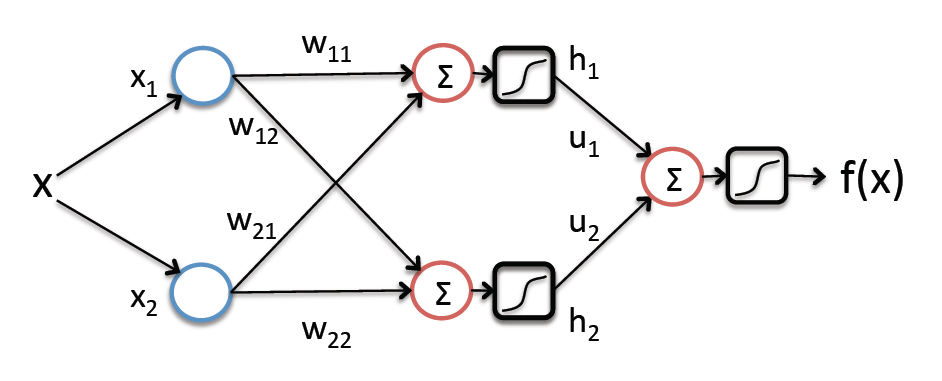
\includegraphics[scale=0.27]{image/neural_net_1.png}
\vspace{-0.1in}
\caption{Illustration of Simple Neural Network.}
\label{fig:neuralnet}
\end{figure}

In this question, we will consider the following neural network depicted in Figure \ref{fig:neuralnet}.  There are six parameters in the model, $u_1$, $u_2$, $w_{11}$, $w_{21}$, $w_{12}$, and $w_{22}$.

The network takes in a 2-dimensional input $x$ and outputs a real value $f(x) \in [0,1]$.  The final output $f(x)$ is a weighted combination of two hidden node activations with a sigmoid transfer function:
\begin{eqnarray}
f(x) = \sigma \left(\sum_{i=1}^2 u_i h_i(x) \right),
\end{eqnarray}
where:
$$\sigma(s) = \frac{e^s}{1+e^s},\ \ \ \ \ \ \ \ \ \ \ \mbox{and}\ \ \ \ \ \ \ \ \ \ \ \ 
h_i(x) = \sigma\left(\sum_{j=1}^2 w_{ji} x_j\right).$$

\smallskip

\textbf{Question 1:} (5 points)
For a given training data point $(x,y)$, compute the stochastic gradient of the squared-loss of $(x,y)$ w.r.t. $w_{11}$:
$$\frac{\partial}{\partial w_{11}} L(y,f(x)) \equiv \frac{\partial}{\partial w_{11}}\left(y - f(x)\right)^2.$$

Hint: write the formula using the chain rule and use the following definition of the derivative of $\sigma(s)$:
$$\frac{\partial}{\partial s}  \sigma(s) = \sigma(s)(1-\sigma(s)).$$
\bigskip

\textbf{Question 2:} (5 points)
Find $\frac{\partial}{\partial w_{11}} L(y,f(x))$ where:
$$(x, y) = ((0.1, 0.5), 0.75)$$
$$(u_1, u_2) = (0.5, -0.1)$$
$$(w_{11}, w_{12}, w_{21}, w_{22}) = (0.25, 0.1, 0.05, -0.25)$$
\smallskip

\textbf{Question 3:}  (5 points)
Use your derivations from the previous two questions to identify which term in the gradient derivation results in the vanishing gradient problem, and briefly explain how the problem is exacerbated in neural networks with more layers.
\smallskip




\end{document}
